
\section*{Problem 2}

\begin{problem}{A.}
\vspace{2mm}

We have a hypothetical crystal, whose refractive index depends on both the polarisation and direction of propagation of an incoming EM wave.
\\
Let us choose a Cartesian reference frame, where the boundary between the medium we are investigating and vacuum is $x=0$ plane. The incident wave, lies in the xy plane, having a wave vector $\vec{k}_i$, making an angle $\theta_i$ with the $x-\mathrm{axis}$ (As shown in the  figure). Let us define two polarisations, S and P. Where S polarisation is when the wave is polarised perpendicular to the incident $xy$ plane and P is the polarisation when the electric field of the wave lies in the xy plane. Let us assume two real and positive refractive indices for S and P waves $\eta_S$ and $\eta_P$ repectively. Without loss of generality assume $\eta_P>\eta_S$.
\\
Say the incoming wave is linearly polarised confined in the $xy$ plane, with its electric field making an angle $\frac{\pi}{4}$ with the $z$ axis. This wave is a mixture of both $S$ and $P$ polarisation. It splits into two at different angles $\theta_{t\pm}=\theta_t \pm \alpha$, where $\vec{k}_{t+}$ corresponds to S, and $\vec{k}_{t-}$ corresponds to P. 
\end{problem}
\begin{center}
    

\tikzset{every picture/.style={line width=0.75pt}} %set default line width to 0.75pt        

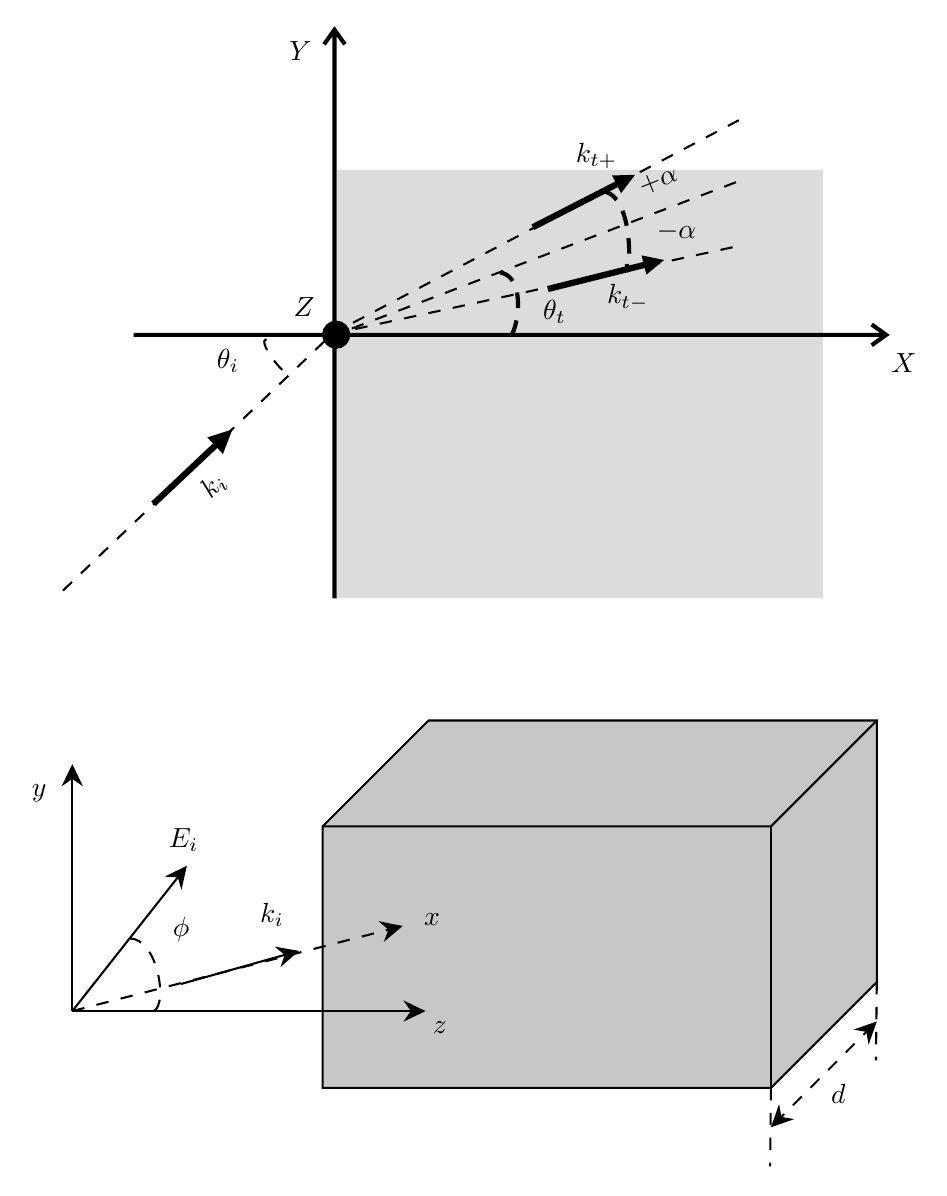
\begin{tikzpicture}[x=0.75pt,y=0.75pt,yscale=-1,xscale=1]
%uncomment if require: \path (0,606); %set diagram left start at 0, and has height of 606

%Shape: Rectangle [id:dp41394729732408253] 
\draw  [draw opacity=0][fill={rgb, 255:red, 155; green, 155; blue, 155 }  ,fill opacity=0.35 ] (251.13,82.37) -- (485.49,82.37) -- (485.49,289) -- (251.13,289) -- cycle ;
%Shape: Axis 2D [id:dp26172173283960065] 
\draw [line width=1.5]  (153.17,162) -- (515.81,162)(250,15) -- (250,289) (508.81,157) -- (515.81,162) -- (508.81,167) (245,22) -- (250,15) -- (255,22)  ;
%Straight Lines [id:da8337450025284996] 
\draw  [dash pattern={on 4.5pt off 4.5pt}]  (119.17,285.2) -- (247.17,163.2) ;
%Curve Lines [id:da1405822884062613] 
\draw  [dash pattern={on 4.5pt off 4.5pt}]  (217.13,164) .. controls (212.3,164.95) and (226.77,183.09) .. (227.5,180.02) ;
%Straight Lines [id:da479198997901781] 
\draw [line width=2.25]    (162.74,243.46) -- (197.17,211) ;
\draw [shift={(200.81,207.57)}, rotate = 136.68] [fill={rgb, 255:red, 0; green, 0; blue, 0 }  ][line width=0.08]  [draw opacity=0] (11.43,-5.49) -- (0,0) -- (11.43,5.49) -- cycle    ;
%Straight Lines [id:da6299546920152124] 
\draw [line width=0.75]  [dash pattern={on 4.5pt off 4.5pt}]  (248.32,161.72) -- (444.81,58.57) ;
%Straight Lines [id:da3883728648151408] 
\draw [line width=0.75]  [dash pattern={on 4.5pt off 4.5pt}]  (247.17,163.2) -- (444.81,87.93) ;
%Straight Lines [id:da4998060156867363] 
\draw [line width=0.75]  [dash pattern={on 4.5pt off 4.5pt}]  (248.32,161.72) -- (445.81,118.93) ;
%Curve Lines [id:da6470768122125261] 
\draw [line width=1.5]  [dash pattern={on 5.63pt off 4.5pt}]  (379.8,92.91) .. controls (395.81,95.93) and (391.81,139.93) .. (390.81,127.93) ;
%Curve Lines [id:da8038047661899634] 
\draw [line width=1.5]  [dash pattern={on 5.63pt off 4.5pt}]  (329.8,131.91) .. controls (338.32,133.52) and (339.19,144.75) .. (337.99,153.1) .. controls (336.93,160.44) and (334.27,165.54) .. (333.81,159.93) ;
%Straight Lines [id:da4217023866157301] 
\draw [line width=2.25]    (345.56,110.14) -- (390.35,87.19) ;
\draw [shift={(394.8,84.91)}, rotate = 152.87] [fill={rgb, 255:red, 0; green, 0; blue, 0 }  ][line width=0.08]  [draw opacity=0] (10,-4.8) -- (0,0) -- (10,4.8) -- cycle    ;
%Straight Lines [id:da49843178394801124] 
\draw [line width=2.25]    (352.81,139.93) -- (403.95,127.14) ;
\draw [shift={(408.81,125.93)}, rotate = 165.96] [fill={rgb, 255:red, 0; green, 0; blue, 0 }  ][line width=0.08]  [draw opacity=0] (10,-4.8) -- (0,0) -- (10,4.8) -- cycle    ;
%Shape: Circle [id:dp03983391745542253] 
\draw  [fill={rgb, 255:red, 0; green, 0; blue, 0 }  ,fill opacity=1 ] (244.51,161.93) .. controls (244.51,158.46) and (247.33,155.64) .. (250.81,155.64) .. controls (254.28,155.64) and (257.1,158.46) .. (257.1,161.93) .. controls (257.1,165.41) and (254.28,168.22) .. (250.81,168.22) .. controls (247.33,168.22) and (244.51,165.41) .. (244.51,161.93) -- cycle ;
%Shape: Cube [id:dp6684229072869232] 
\draw  [fill={rgb, 255:red, 0; green, 0; blue, 0 }  ,fill opacity=0.22 ] (244.28,398.8) -- (295.28,347.8) -- (511.28,347.8) -- (511.28,473.8) -- (460.28,524.8) -- (244.28,524.8) -- cycle ; \draw   (511.28,347.8) -- (460.28,398.8) -- (244.28,398.8) ; \draw   (460.28,398.8) -- (460.28,524.8) ;
%Straight Lines [id:da7498729323670823] 
\draw    (123.68,487.8) -- (123.68,371.8) ;
\draw [shift={(123.68,368.8)}, rotate = 90] [fill={rgb, 255:red, 0; green, 0; blue, 0 }  ][line width=0.08]  [draw opacity=0] (10.72,-5.15) -- (0,0) -- (10.72,5.15) -- (7.12,0) -- cycle    ;
%Straight Lines [id:da8208999367418137] 
\draw    (123.68,487.8) -- (290.88,487.8) ;
\draw [shift={(293.88,487.8)}, rotate = 180] [fill={rgb, 255:red, 0; green, 0; blue, 0 }  ][line width=0.08]  [draw opacity=0] (10.72,-5.15) -- (0,0) -- (10.72,5.15) -- (7.12,0) -- cycle    ;
%Straight Lines [id:da7174552504343465] 
\draw    (123.68,487.8) -- (177.03,420.16) ;
\draw [shift={(178.88,417.8)}, rotate = 128.26] [fill={rgb, 255:red, 0; green, 0; blue, 0 }  ][line width=0.08]  [draw opacity=0] (10.72,-5.15) -- (0,0) -- (10.72,5.15) -- (7.12,0) -- cycle    ;
%Straight Lines [id:da21779076116998253] 
\draw  [dash pattern={on 4.5pt off 4.5pt}]  (123.68,487.8) -- (279.98,447.55) ;
\draw [shift={(282.88,446.8)}, rotate = 165.56] [fill={rgb, 255:red, 0; green, 0; blue, 0 }  ][line width=0.08]  [draw opacity=0] (10.72,-5.15) -- (0,0) -- (10.72,5.15) -- (7.12,0) -- cycle    ;
%Straight Lines [id:da4538137858169531] 
\draw    (175.88,474.8) -- (230,459.61) ;
\draw [shift={(232.88,458.8)}, rotate = 164.32] [fill={rgb, 255:red, 0; green, 0; blue, 0 }  ][line width=0.08]  [draw opacity=0] (10.72,-5.15) -- (0,0) -- (10.72,5.15) -- (7.12,0) -- cycle    ;
%Curve Lines [id:da5782358459753356] 
\draw  [dash pattern={on 4.5pt off 4.5pt}]  (151.28,452.8) .. controls (164.88,452.8) and (169.88,484.8) .. (162.88,487.8) ;

%Straight Lines [id:da995607271595156] 
\draw  [dash pattern={on 4.5pt off 4.5pt}]  (460.28,524.8) -- (459.96,555.61) -- (459.88,562.6) ;
%Straight Lines [id:da22758558142862872] 
\draw  [dash pattern={on 4.5pt off 4.5pt}]  (511.28,473.8) -- (511.12,489.63) -- (510.97,503.6) -- (510.88,511.6) ;
%Straight Lines [id:da17388485750558225] 
\draw  [dash pattern={on 4.5pt off 4.5pt}]  (462.41,541.68) -- (509.16,494.92) ;
\draw [shift={(511.28,492.8)}, rotate = 135] [fill={rgb, 255:red, 0; green, 0; blue, 0 }  ][line width=0.08]  [draw opacity=0] (10.72,-5.15) -- (0,0) -- (10.72,5.15) -- (7.12,0) -- cycle    ;
\draw [shift={(460.28,543.8)}, rotate = 315] [fill={rgb, 255:red, 0; green, 0; blue, 0 }  ][line width=0.08]  [draw opacity=0] (10.72,-5.15) -- (0,0) -- (10.72,5.15) -- (7.12,0) -- cycle    ;
% Text Node
\draw (102.68,377.2) node [anchor=north west][inner sep=0.75pt]    {${y}$};
% Text Node
\draw (295.88,491.2) node [anchor=north west][inner sep=0.75pt]    {${z}$};
% Text Node
\draw (291.68,439.2) node [anchor=north west][inner sep=0.75pt]    {${x}$};
% Text Node
\draw (212.68,434.2) node [anchor=north west][inner sep=0.75pt]    {${k_{i}}$};
% Text Node
\draw (168.68,398.2) node [anchor=north west][inner sep=0.75pt]    {${E_{i}}$};
% Text Node
\draw (170.68,441.2) node [anchor=north west][inner sep=0.75pt]    {$\phi$};
% Text Node
\draw (487.78,521.7) node [anchor=north west][inner sep=0.75pt]    {${d}$};
% Text Node
\draw (516.8,169.31) node [anchor=north west][inner sep=0.75pt]    {${X}$};
% Text Node
\draw (226.8,19.31) node [anchor=north west][inner sep=0.75pt]    {${Y}$};
% Text Node
\draw (379.8,136.31) node [anchor=north west][inner sep=0.75pt]    {${k_{t-}}$};
% Text Node
\draw (403.8,106.31) node [anchor=north west][inner sep=0.75pt]    {$-\alpha $};
% Text Node
\draw (393.62,86.13) node [anchor=north west][inner sep=0.75pt]  [rotate=-338.35]  {$+\alpha $};
% Text Node
\draw (364.8,68.31) node [anchor=north west][inner sep=0.75pt]    {${k_{t+}}$};
% Text Node
\draw (349.06,143.73) node [anchor=north west][inner sep=0.75pt]    {${\theta }_{t}$};
% Text Node
\draw (191.8,167.4) node [anchor=north west][inner sep=0.75pt]    {${\theta _{i}}$};
% Text Node
\draw (181.7,234.84) node [anchor=north west][inner sep=0.75pt]  [rotate=-314.46]  {${k_{i}}$};
% Text Node
\draw (228.8,142.4) node [anchor=north west][inner sep=0.75pt]    {$Z$};


\end{tikzpicture}

\end{center}
\newpage
\begin{subpr}{A1. \hfill 1.5 pts.} Find $n_S$  and $n_P$ in terms of $\theta_t$, $\theta_i$, $\alpha$. Assume that $n_S=n_0+\Delta n$ and $n_P=n_0-\Delta n$, where $\Delta n/n_0 <<1$ and we only look for first-order terms in $\Delta n/n_0$.
\end{subpr}
\begin{problem}{}
 Now assume the incidence to be normal, and the electric field still makes an angle $\pi/4$ with the $z$-axis (As can be seen in the figure). The crystal has a thickness $t>>\lambda$. 
\end{problem}
\begin{subpr}{A2. \hfill 1 pts.} Find the values of $t$ for which the light exiting crystal is either circularly polarised or it is linearly polarised, but rotated by and angle $\pi/2$ with respect to the incident polarisation. You may neglect the difference between Reflection coefficients for $S$ and $P$.
\end{subpr}

\begin{problem}{B.}
 Let us investigate a plane EM wave, of frequency $\omega$ travelling in a static uniform magnetic field $B_0 \hat{z}$, where $\hat{z}$ is the unit vector $z$ of the chosen Cartesian frame of reference. $B_0$ is much stronger than the field of the wave and the wave propagation is also along $\hat{z}$. 
\\
 This medium contains $N_e$ bound electrons per unit volume, each obeying the classical equation of motion.
 \begin{equation}
e(\vec{E}+\frac{\vec{v}}{c}\times \vec{B}) +m_e \omega^2 r= -m_e \ddot{\vec{r}}, \vec{v}=\frac{d\vec{r}}
{dt}\end{equation}
Where $m_e$ and $-e$ are the mass and charge of electron respectively.
\end{problem}
\begin{subpr}{B1. \hfill 4.5 pts.} Prove that the wave propagation depends on polarisation, by calculating the refractive index for circular polarisation  (either left handed or right).
\end{subpr}
\begin{problem}{}
Now consider the propagation of a linearly polarised in the same wave. Asuume the field at $z=0$ to be given by $\vec{E}_i (z=0,t)=E_i e^{-i\omega t} \hat{x}$, and a relatively weak magnetic field such that $\omega >> \omega_c$ and higher order terms of $\omega_c/\omega$ can be neglected.
\end{problem}
\begin{subpr}{B2. \hfill 3 pts.} Calculate the electric field at $z=l$, and find the angle by which the polarization has rotated.
\end{subpr}
\clearpage